%\documentclass[mathserif]{beamer}
\documentclass[handout]{beamer}
%\usetheme{Goettingen}
\usetheme{Warsaw}
%\usetheme{Singapore}
%\usetheme{Frankfurt}
%\usetheme{Copenhagen}
%\usetheme{Szeged}
%\usetheme{Montpellier}
%\usetheme{CambridgeUS}
%\usecolortheme{}
%\setbeamercovered{transparent}
\usepackage[english, activeacute]{babel}
\usepackage[utf8]{inputenc}
\usepackage{amsmath, amssymb}
\usepackage{dsfont}
\usepackage{graphics}
\usepackage{cases}
\usepackage{graphicx}
\usepackage{pgf}
\usepackage{epsfig}
\usepackage{amssymb}
\usepackage{multirow}	
\usepackage{amstext}
\usepackage[ruled,vlined,lined]{algorithm2e}
\usepackage{amsmath}
\usepackage{epic}
\usepackage{epsfig}
\usepackage{fontenc}
\usepackage{framed,color}
\usepackage{palatino, url, multicol}
\usepackage{listings}
%\algsetup{indent=2em}
\newcommand{\factorial}{\ensuremath{\mbox{\sc Factorial}}}
\newcommand{\BIGOP}[1]{\mathop{\mathchoice%
{\raise-0.22em\hbox{\huge $#1$}}%
{\raise-0.05em\hbox{\Large $#1$}}{\hbox{\large $#1$}}{#1}}}
\newcommand{\bigtimes}{\BIGOP{\times}}
\vspace{-0.5cm}
\title{Probability}
\vspace{-0.5cm}
\author[Felipe Bravo Márquez]{\footnotesize
%\author{\footnotesize  
 \textcolor[rgb]{0.00,0.00,1.00}{Felipe José Bravo Márquez}} 
\date{ \today }


\begin{document}
\begin{frame}
\titlepage


\end{frame}


%%%%%%%%%%%%%%%%%%%%%%%%%%%

\begin{frame}{Probability and Statistics}

\scriptsize{
\begin{itemize}
 \item Probability is the language of \textbf{uncertainty} that is also the basis for statistical inference \cite{poldrack2019statistical}. 

 \item It forms an important part of the foundation for statistics, because it provides us with the mathematical tools to describe uncertain events. 
 \item The study of probability arose in part due to interest in understanding games of chance, like cards or dice. 
 \item These games provide useful examples of many statistical concepts, because when we repeat these games the likelihood of different outcomes remains (mostly) the same.
\end{itemize}

\begin{figure}[h!]
	\centering
	
\includegraphics[scale=0.2]{pics/gambling.png}
\end{figure}


}

\end{frame}


\begin{frame}{Probability and Statistics}

\scriptsize{
\begin{itemize}
  \item The problem studied in probabilities is: given a data generating process, which are the properties of the outputs?
 \item The problem studied in statistical inference, data mining and machine learning is: given the outputs, what can we say about the process that generates the observed data? 
\end{itemize}

}
\begin{figure}[h!]
	\centering
	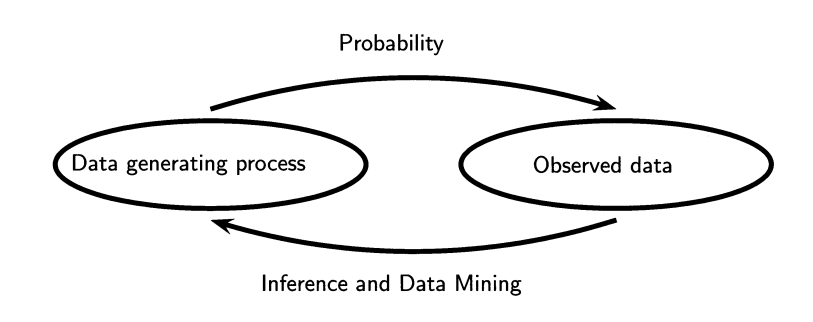
\includegraphics[scale=0.3]{pics/probandstats.png}
\end{figure}

\footnotemark{Figure taken from \cite{wasserman2013all}}

\end{frame}

\begin{frame}\frametitle{What is Probability?}
\scriptsize{

\begin{itemize}
 \item We think of probability as a number that describes the likelihood of some event occurring, which ranges from zero (impossibility) to one (certainty).
 \item Probabilities can also be expressed in percentages: when the weather forecast predicts a twenty percent chance of rain today. 
 \item In each case, these numbers are expressing how likely that particular event is, ranging from absolutely impossible to absolutely certain.
\end{itemize}

}

\end{frame}



\begin{frame}\frametitle{Probability Concepts}
\scriptsize{

\begin{itemize}
 \item A \textbf{random experiment} in the act of measuring a process whose output is uncertain. 
 \item Examples: flipping a coin, rolling a 6-sided die, or trying a new route to work to see if it’s faster than the old route.
 \item The set with all possible outputs of a random experiment is the \textbf{sample space} $\Omega$ (it can be discrete or continuous).
 \item For a coin flip  $\Omega = \{$heads, tails$\}$, for the 6-sided die  $\Omega = \{1,2,3,4,5,6\}$, and  for the amount of time it takes to get to work $\Omega$ is all possible real numbers greater than zero.
 \item An \textbf{event} $E \subseteq \Omega$ corresponds to a subset of those outputs.
 \item For example, $E = \{ 2,4,6 \}$ is the event of observing an even number when rolling a die.
\end{itemize}

}

\end{frame}

\begin{frame}\frametitle{Probability}
\begin{scriptsize}
\begin{itemize}
\item Now we can outline the formal features of a probability, which were first defined by the Russian mathematician Andrei Kolmogorov.
\begin{figure}[h!]
	\centering
	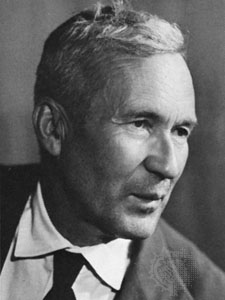
\includegraphics[scale=0.15]{pics/kolmogorov.jpeg}
\end{figure}



 \item A probability $\mathbb{P}$ is a real-valued function defined over $\Omega$ that satisfies the following properties:
\end{itemize}

\begin{block}{Properties}
\begin{enumerate}
 \item For any event $E \subseteq \Omega$ , $0 \leq \mathbb{P}(E) \leq 1$.
 \item The probability of the sample space is 1: $\mathbb{P}(\Omega) =1$
 \item Let $E_{1},E_{2},\dots,E_{k} \in \Omega$ be disjoint sets 
 \begin{displaymath}
  \mathbb{P}(\bigcup_{i=1}^{k}E_{i}) = \sum_{i}^{k}P(E_{i})
 \end{displaymath}
\end{enumerate}
\end{block}

Probabilities cannot be negative or greater than 1.

\end{scriptsize} 

\end{frame}


\begin{frame}\frametitle{Interpretation of Probabilities}
\begin{scriptsize}
\begin{itemize}
\item The are two common interpretations of probabilities: frequencies and degrees of beliefs. 
\item In the frequency interpretation, $\mathbb{P}(E)$ is the long run proportion of times that $E$ is true in repetitions. 
\item For example, if we say that the probability of heads is 1/2, we mean that if we flip the coin many times then the proportion of times we get heads tends to 1/2 as the number of tosses increases. 
\item The degree-of-belief interpretation is that $\mathbb{P}(E)$ measures an observer's strength of belief that $E$ is true.
\item In either interpretation, we require that properties 1 to 3 hold. 
\item The difference in interpretation will not matter much until we deal with statistical inference. 
\item There, the differing interpretations lead to two schools of inference: the frequentist and the Bayesian schools.
\end{itemize}


\end{scriptsize} 

\end{frame}


\begin{frame}{Random Variable}
\scriptsize{

\begin{itemize}
 \item A \textbf{random variable} is a mapping (or function)
\begin{displaymath}
 X: \Omega \rightarrow \mathbb{R}
\end{displaymath}
which assigns a real value $X(e)$ to any event of $\Omega$.


\item Example: We flip a fair coin 10 times. The outcome of each toss is a head $H$ or a tail $T$.

\item  Let $X(e)$ be the number of heads in the sequence of outcomes.
\begin{itemize}
 \item If $e=HHTHHTHHTT$, then $X(e)=6$ 
\end{itemize}


\end{itemize}

}

\end{frame}

\begin{frame}{Ejemplo}

\begin{itemize}
 \item Tiramos una moneda 2 veces. Sea $X$ la la cantidad de sellos obtenidos.
 \item La variable aleatoria y su distribución se resume como:
\end{itemize}

\begin{table}
\begin{tabular}{c c|c}
\hline
 $e$ & $\mathbb{P}(e)$ & $X(e)$   \\ 
\hline
CC & 1/4 & 0 \\
CS & 1/4 & 1 \\
SC & 1/4 & 1 \\
SS & 1/4 & 2 \\
\hline
\end{tabular}
\end{table}

\begin{table}
\begin{tabular}{c|c}
\hline
 $x$ & $\mathbb{P}(X = x)$   \\ 
\hline
0 & 1/4 \\
1 & 1/2  \\
2 & 1/4  \\
\hline
\end{tabular}
\end{table}

\end{frame}




\begin{frame}{Definiciones de V.A}
\scriptsize{
\begin{itemize}
 \item Sea $X$ una V.A , se define \textbf{función de distribución acumulada} (CDF) o \ $F_{X}: \mathbb{R} \rightarrow [0,1]$
\begin{displaymath}
 F_{X}(x)=\mathbb{P}(X\leq x)
\end{displaymath}
\end{itemize}

\begin{block}{Variables Aleatorias Discretas}
\begin{itemize}
\item Una V.A $X$ es \textbf{discreta} si mapea las salidas a un conjunto contable.
\item Se define la \textbf{función de probabilidad} o \textbf{función de masa de probabilidad} de una V.A $X$ discreta como $f_{X}(x)=\mathbb{P}(X=x)$
\item Entonces $f_{X}(x) \geq 0$  $\forall x \in \mathbb{R}$ y $\sum_{i}f_{X}(x_{i})=1$
\item La CDF de $X$ se relaciona con $f_{X}$ de la siguiente manera: 
\begin{displaymath}
F_{X}= \mathbb{P}(X\leq x)= \sum_{x_{i} \leq x} f_{X}(x_{i})  
\end{displaymath}
  
\end{itemize}
 
\end{block}



} 
\end{frame}

\begin{frame}{Definiciones de V.A II}
\scriptsize{
\begin{block}{Variable Aleatoria continua}
\begin{itemize}
 \item Una V.A $X$ es continua si:
 \item existe una función $f_{X}$ tal que $f_{X}(x) \geq 0$ $\forall x$,  $\int_{-\infty}^{\infty}f_{X}(x)dX=1$
 \begin{displaymath}
      \int_{-\infty}^{\infty}f_{X}(x)dX=1
       \end{displaymath}
\item Para todo $a \geq b$:
\begin{displaymath}
 \mathbb{P}(a < X < b) = \int_{a}^{b} f_{X}(x)dx
\end{displaymath}
\end{itemize}

\end{block}

\begin{itemize}
 \item La función $f_{X}$ recibe el nombre de \textbf{función densidad de probabilidad} (PDF). 
 \item La PDF se relaciona con la CDF como:
 \begin{displaymath}
 F_{X}(x)=\int_{-\infty}^{x}f_{X}(t)dt 
 \end{displaymath}
\item Luego $f_{X}(x) = F'_X(x)$ en todos los puntos $x$ donde $F_{X}$ es diferenciable
\item Para distribuciones continuas la probabilidad que $X$ tomo un \textbf{valor particular} vale siempre \textbf{cero}.

\end{itemize}




}
\end{frame}

\begin{frame}{Algunas Propiedades}

\begin{enumerate}
 \item $ \mathbb{P}( x < X \leq y) = F(y) - F(x)$
       

\item $ \mathbb{P}(X > x) = 1 - F(x)$ 

\item Si $X$ es continua luego 
\begin{eqnarray*}
 F(b) - F(a) = \mathbb{P}(a < X < b) = \mathbb{P} ( a \leq X < b)  \\
   = \mathbb{P} ( a < X \leq b) = \mathbb{P} ( a \leq X \leq b) 
\end{eqnarray*}

\end{enumerate}



 
\end{frame}



\begin{frame}{Cuantiles}
\scriptsize{
\begin{itemize}
 \item Sea $X$ una V.A con CDF $F$. La CDF inversa o función cuantía se define como \begin{displaymath}
                                                                                   F^{-1}(q)= inf \left\{ x: \ F(x) > q \right\}
                                                                                     \end{displaymath}
 \item Para $q \in [0,1]$ si $F$ es estrictamente creciente y continua, $F^{-1}(q)$ es el único valor real tal que $F(x)=q$
 \item Luego $F^{-1}(1/4)$ es l primer cuartil, $F^{-1}(1/2)$ la mediana (o segundo cuartil) y $F^{-1}(3/4)$ el tercer cuartil.
 
 
\end{itemize}

}

\end{frame}




\begin{frame}{Algunas distribuciones}
\scriptsize{ 

\begin{table}
\centering
\begin{tabular}{c|c|c}
\hline
  & Función de Probabilidad & Parámetros   \\ 
\hline
Normal & $f_x=\frac{1}{\sqrt{2\pi}\sigma}\exp^{-\frac{1}{2}\frac{(x-\mu)^2}{\sigma^{2}}}$ & $\mu, \sigma$ \\ \hline
Binomial & $f_x= {n \choose x}p^{x}(1-p)^{n-x} $ & $n,p$ \\ \hline
Poisson & $f_x=\frac{1}{x!}\lambda^{x}\exp^{-\lambda}$ & $\lambda$ \\ \hline
Exponencial & $f_x= \lambda \exp^{-\lambda x}$  & $\lambda$ \\ \hline
Gamma & $f_x= \frac{\lambda^{\alpha}}{\Gamma(\alpha)} x^{\alpha -1}\exp^{-\lambda x} $ & $\lambda , \alpha$ \\ \hline
Chi-cuadrado & $f_x=\frac{1}{2^{k/2} \Gamma(k/2)} x^{(\frac{k}{2} -1)} \exp^{-x/2} $  & $k$  \\
\hline
\end{tabular}
\end{table}

}
\end{frame}



\begin{frame}{Binomial Distribution}

\scriptsize{
\begin{itemize}
 \item  The binomial distribution is a discrete distribution that provides a way to compute the probability of some number of successes out of a number of trials.
 \item In each trial there is either success or failure and nothing in between (known as “Bernoulli trials”) given some known probability of success on each trial.
 \item Let $n$ be the number of trials, $x$ the number of successes, and $p$ the probability of a success, the probability mass function of the Binomial distribution is as follows:
 \begin{displaymath}
  f_x(n,p)= {n \choose x}p^{x}(1-p)^{n-x} 
 \end{displaymath}
\item The binomial coefficient ${n \choose x}$ describes the number of different ways that one can choose $x$ items out of $n$ total items.
 
 
 \end{itemize}}
 
 \end{frame}
 
 


\begin{frame}{Distribución Normal}

\scriptsize{
\begin{itemize}
 \item $X$ tiene una distribución Normal o Gaussiana de parámetros  $\mu$ y $\sigma$, $X \sim N(\mu,\sigma^2)$ si
 \begin{displaymath}
 f_x=\frac{1}{\sqrt{2\pi}\sigma}\exp^{-\frac{1}{2}\frac{(x-\mu)^2}{\sigma^{2}}} 
 \end{displaymath}
 \item Donde $\mu \in \mathbb{R}$ es el ``centro'' o la \textbf{media} de la distribución y $\sigma > 0$ es la \textbf{desviación estándar}.
 \item Cuando $\mu = 0$ y $\sigma =1$ tenemos una \textbf{Distribución Normal Estándar} denotada por $Z$.
 \item Denotamos por $\phi(z)$ a la PDF y por $\Phi(z)$ a la CDF de una Normal estándar.
 \item Los valores de  $\Phi(z)$, $\mathbb{P}(Z \leq z)$ se encuentran tabulados.
 \end{itemize}

\begin{block}{Propiedades Útiles}
\begin{enumerate}
 \item Si $X \sim N(\mu, \sigma^2)$, luego $Z=(X-\mu)/\sigma \sim N(0,1)$
 \item Si $Z \sim N(0,1)$, luego $X=\mu+\sigma Z \sim N(\mu, \sigma^2)$
 \item Sean $X_{i} \sim N(\mu_{i},\sigma_{i}^{2})$ ,$i=1,\dots,n$ \ V.As independientes:
 \begin{displaymath}
  \sum_{i=1}^{n}X_{i}\sim N( \sum_{i=1}^{n}\mu_{i}, \sum_{i=1}^{n}\sigma_{i}^{2})
 \end{displaymath}

 
\end{enumerate}
 
\end{block}




}
\end{frame}

\begin{frame}[fragile]{Ejemplo Normal}
\scriptsize{
\begin{itemize}
 \item En R podemos acceder a las PDF, CDF, función cuantía y generación de números aleatorios de las distribuciones.
 \item Para una Normal son:
\begin{verbatim}
dnorm(x, mean = 0, sd = 1, log = FALSE)
pnorm(q, mean = 0, sd = 1, lower.tail = TRUE, log.p = FALSE)
qnorm(p, mean = 0, sd = 1, lower.tail = TRUE, log.p = FALSE)
rnorm(n, mean = 0, sd = 1) 
\end{verbatim}
 
\end{itemize}

\begin{block}{Ejemplo}
Sea $X\sim N(3,5)$, encontrar $\mathbb{P}(X > 1)$ \\
$\mathbb{P}(X >1) = 1-\mathbb{P}(X<1) = 1-\mathbb{P}(Z < \frac{1-3}{\sqrt{5}})=1-\Phi(-0.8944)= 0.81$ \\
En R:
\begin{verbatim}
 > 1-pnorm(q=(1-3)/sqrt(5))
[1] 0.8144533
\end{verbatim}
O directamente:
\begin{verbatim}
> 1-pnorm(q=1,mean=3,sd=sqrt(5))
[1] 0.8144533 
\end{verbatim}
\end{block}
}
\end{frame}


\begin{frame}[fragile]{La regla 68-95-99.7 de una Normal}
\scriptsize{
\begin{figure}[h!]
	\centering
	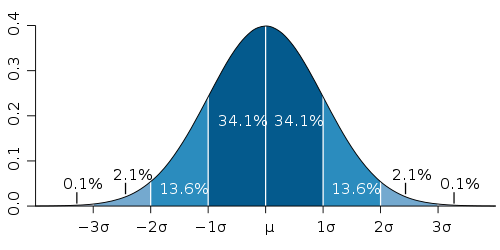
\includegraphics[scale=0.3]{pics/gaussian.png}
\end{figure} 
Sea $X$ una V.A $\sim N(\mu,\sigma^2)$
\begin{itemize}
 \item $\mathbb{P}( \mu - \sigma \leq X \leq \mu+ \sigma) \approx 0.6827$  
 \item $\mathbb{P}( \mu - 2 \sigma \leq X \leq \mu+ 2 \sigma) \approx 0.9545$               
 \item $\mathbb{P}( \mu - 3 \sigma \leq X \leq \mu+ 3 \sigma) \approx 0.9973$ 

\end{itemize}
En R para $X\sim N(0,1)$:
\begin{verbatim}
> pnorm(1)-pnorm(-1)
[1] 0.6826895
> pnorm(2)-pnorm(-2)
[1] 0.9544997
> pnorm(3)-pnorm(-3)
[1] 0.9973002 
\end{verbatim}
}
\end{frame}

\begin{frame}[fragile]{Simetría de la Normal}
\begin{itemize}
 \item La PDF de una normal es simétrica alrededor de $\mu$
 \item Entonces $\phi(z)= \phi(-z) $ 
 \item $\Phi(z)=1-\Phi(-z)$
\end{itemize}
\begin{verbatim}
> dnorm(1)
[1] 0.2419707
> dnorm(-1)
[1] 0.2419707
> pnorm(0.95)
[1] 0.8289439
> 1-pnorm(-0.95)
[1] 0.8289439 
\end{verbatim}


\end{frame}

\begin{frame}[fragile]{Graficando la PDF de Normales con distinta varianza en R}
\scriptsize{
\begin{verbatim}
x=seq(-8,8,length=400)
y1=dnorm(x,mean=0,sd=0.5)
y2=dnorm(x,mean=0,sd=1) 
y3=dnorm(x,mean=0,sd=2)
plot(y1~x,type="l",col="red")
lines(y2~x,type="l",col="green")
lines(y3~x,type="l",col="blue")
\end{verbatim}
}
 \begin{figure}[h!]
	\centering
	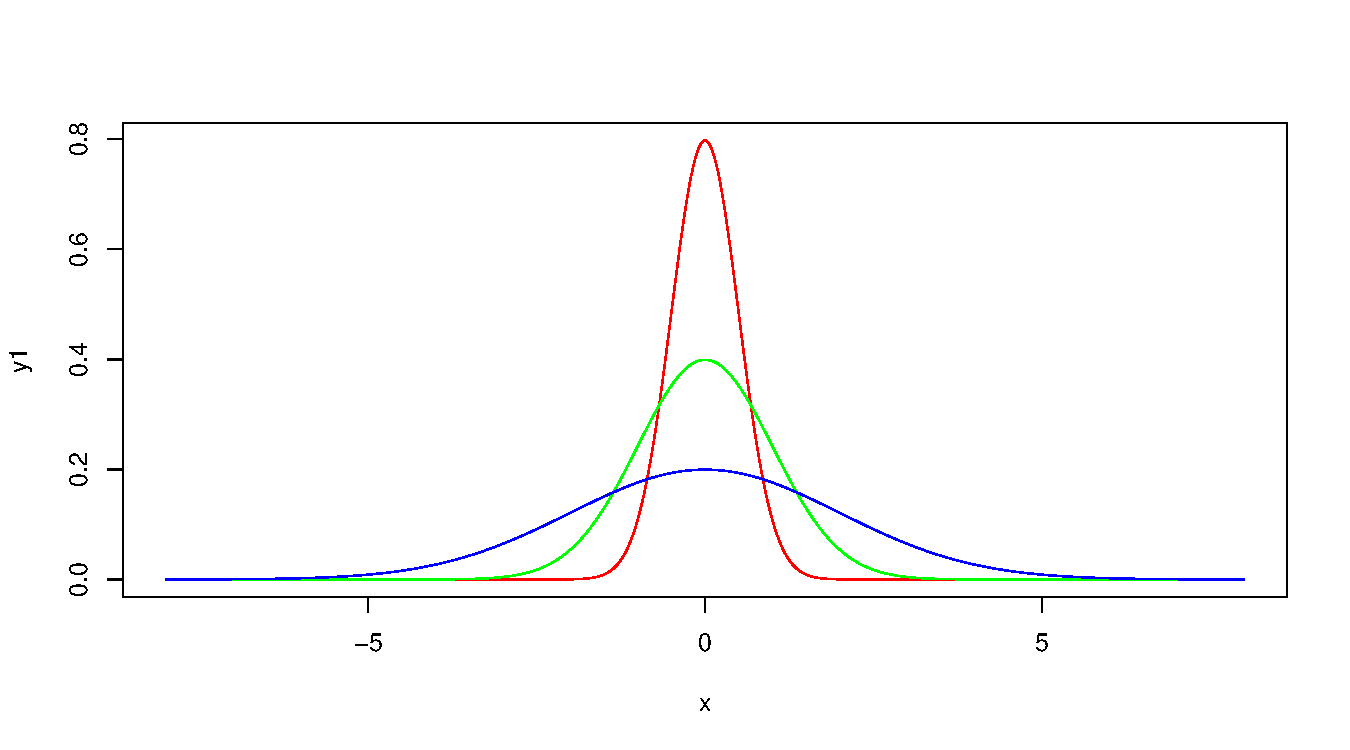
\includegraphics[scale=0.35]{pics/normplot.pdf}
\end{figure}



\end{frame}




\begin{frame}{Probabilidades Conjuntas y Condicionales}
\scriptsize{
\begin{itemize}
 \item La noción de función probabilidad (masa o densidad) se puede \textbf{extender} a más de una V.A 
 \item Sean $X$  $Y$ dos V.A, $\mathbb{P}(X,Y)$ representa la \textbf{función de probabilidad conjunta}.
 \item Las variables son independientes entre sí, si \begin{displaymath}
                                                      \mathbb{P}(X,Y)=\mathbb{P}(X)\times \mathbb{P}(Y)
                                                     \end{displaymath}
\item La \textbf{probabilidad condicional} para $Y$ dado $X$ se define como
 \begin{displaymath}
  \mathbb{P}(Y|X) = \frac{\mathbb{P}(X,Y)}{\mathbb{P}(X)}
 \end{displaymath}
\item Si $X$ e $Y$ son independientes $\mathbb{P}(Y|X)=\mathbb{P}(Y)$
\end{itemize}




} 
\end{frame}


\begin{frame}{Probabilidades Conjuntas y Condicionales (2)}
 \begin{figure}[h!]
	\centering
	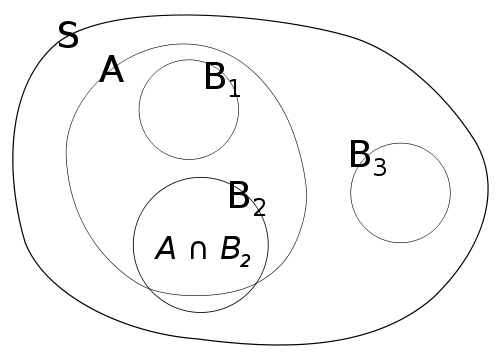
\includegraphics[scale=0.3]{pics/condicional.png}
	\caption{Fuente: \url{en.wikipedia.org/wiki/Conditional_probability}}
\end{figure}



\scriptsize{
\begin{itemize}
 \item Sea $S$ el espacio muestral, $A$ y $B_n$ eventos.
 \item Las probabilidades son proporcionales al área.
 \item $\mathbb{P}(A) \sim 0.33$, $\mathbb{P}(A|B_1)=1$
 \item $\mathbb{P}(A|B_2)\sim 0.85$ y $\mathbb{P}(A|B_3)=0$ 
\end{itemize}




} 
\end{frame}




\begin{frame}{Teorema de Bayes y Probabilidades Totales}
\scriptsize{
\begin{itemize}
 \item La probabilidad condicional $\mathbb{P}(Y|X)$ y $\mathbb{P}(X|Y)$ pueden ser expresadas en función de la otra usando el \textbf{teorema de Bayes}
\begin{displaymath}
 \mathbb{P}(Y|X)=\frac{\mathbb{P}(X|Y)\mathbb{P}(Y)}{\mathbb{P}(X)}
\end{displaymath}
\item Se entiende a $P(Y|X)$ como la fracción  de veces que $Y$ ocurre cuando se sabe que ocurre $X$.
\item Luego sea $\{ Y_1,Y_2,\dots, Y_k \} $ un conjunto de salidas mutuamente excluyentes de una V.A $X$, el denominador del teorema de Bayes se puede expresar como:
\begin{displaymath}
\mathbb{P}(X)= \sum_{i=1}^{k} \mathbb{P}(X,Y_i) = \sum_{i=1}^{k} \mathbb{P}(X|Y_i)\mathbb{P}(Y_i)
\end{displaymath}
\end{itemize}
 
}
\end{frame}

\begin{frame}{Ejemplo}
\scriptsize{
\begin{itemize}
 \item Divido mis correos en tres categorías: $A_1$=``spam'', $A_2$=``baja prioridad'', $A_3$=``alta prioridad''
 \item Sabemos que $\mathbb{P}(A_1)=0.7$, $\mathbb{P}(A_2)=0.2$ y $\mathbb{P}(A_3)=0.1$, claramente $0.7+0.2+0.1=1$
 \item Sea $B$ el evento de que el correo contenga la palabra ``gratis''.
 \item Sabemos que $\mathbb{P}(B|A_1)=0.9$ $\mathbb{P}(B|A_2)=0.01$ y $\mathbb{P}(B|A_3)=0.01$ claramente $0.9+0.01+0.01 \neq 1$
 \item Cual es la probabilidad de que sea ``spam'' un correo que tiene la palabra ``gratis''?
 \item Usando Bayes y Probabilidades totales:
 \begin{displaymath}
  \mathbb{P}(A_1|B) = \frac{0.9 \times 0.7}{(0.9 \times 0.7) + (0.01 \times 0.2) + (0.01 \times 0.1)} = 0.995
 \end{displaymath}



\end{itemize}




} 
\end{frame}





\begin{frame}{Esperanza}
\scriptsize{
\begin{itemize}
 \item Sea $X$ una V.A, se define su \textbf{esperanza} o \textbf{momento de primer orden} como:
  \begin{displaymath}
  \mathbb{E}(X) = \left\{ \begin{array}{rl}
  \sum_{x}(x\times f(x)) &\mbox{ Si $X$ es discreta} \\
   \int_{-\infty}^{\infty}(x\times f(x))dx &\mbox{ Si $X$ es continua}
       \end{array} \right.
  \end{displaymath}
\item Es el promedio ponderado de todos los posibles valores que puede tomar una variable aleatoria

\item Para el caso de lanzar dos veces una moneda con $X$ el número de caras:
 \begin{eqnarray*}
  \mathbb{E}(X) & = & (0 \times f(0)) + (1 \times f(1)) + (2 \times f(2)) \nonumber \\
       & = & (0 \times (1/4)) + (1 \times (1/2)) + (2 \times (1/4)) =1  \nonumber \\
 \end{eqnarray*}


\item Sean las variables aleatorias $X_1, X_2, \dots , X_n$ y las constantes $a_1, a_2, \dots, a_n$,
\begin{displaymath}
 \mathbb{E}\left(\sum_{i}a_i X_i \right) = \sum_{i} a_{i} \mathbb{E}(X_i)
\end{displaymath}
 


\end{itemize}
}

\end{frame}


\begin{frame}{Varianza}
\scriptsize{
\begin{itemize}
 \item La varianza mide la ``dispersión'' de una distribución
 \item Sea $X$ una V.A de media $\mu$, se define la varianza de $X$ denotada como $\sigma^2$, $\sigma^{2}_{X}$ o $\mathbb{V}(X)$ como:
  \begin{displaymath}
  \mathbb{V}(X) = \mathbb{E}(X - \mu)^2 =  \left\{ \begin{array}{rl}
  \sum_{i=1}^{n} f_{x}(x_{i})(x_{i} - \mu)^2 &\mbox{ Si $X$ es discreta} \\
   \int (x- \mu)^{2}f_X(x)dx &\mbox{ Si $X$ es continua}
       \end{array} \right.
  \end{displaymath}
\item La \textbf{desviación estándar} $\sigma$ se define como $\sqrt{\mathbb{V}(X)}$ 
\end{itemize}

\begin{block}{Propiedades}
\begin{itemize}
\item $\mathbb{V}(X)=  \mathbb{E}(X^2)- \mathbb{E}(X)^2 =  \mathbb{E}(X^2)-\mu^2 $ 
\item Si $a$ y $b$ son constantes, luego $\mathbb{V}(aX+b)=a^2\mathbb{V}(X)$
\item Si $X_1,\dots,X_n$ son independientes y $a_1,\dots,a_n$ son constantes, luego
\begin{displaymath}
 \mathbb{V}\left(\sum_{i=1}^{n}a_i X_i \right) = \sum_{i=1}^{n} a_{i}^{2} \mathbb{V}(X_{i})
\end{displaymath}


\end{itemize}

 
\end{block}


}
\end{frame}



\begin{frame}{Ley de los Grandes Números}
\scriptsize{
\begin{block}{Forma Débil}
\begin{itemize}
 \item Sean $X_{1},X_{2},\dots X_{n}$ variables aleatorias IID de media $\mu$ y varianza $\sigma^2$
 \item El promedio $\overline{X_{n}} =\frac{\sum_{i=1}^{n}X_{i}}{n}$ converge en probabilidad a $\mu$, $\overline{X_{n}} \overset{P}{\rightarrow} \mu$   
 \item Esto es equivalente a decir que para todo $\epsilon > 0$
 \begin{displaymath}
  \lim_{n\rightarrow \infty} \mathbb{P}(|\overline{X_{n}} - \mu| < \epsilon)=1
 \end{displaymath}
\item Entonces la distribución de $\overline{X_{n}}$ se concentra alrededor de $\mu$ cuando $n$ crece.
\end{itemize}
\end{block}
\begin{block}{Ejemplo}
\begin{itemize}
 \item Sea el experimento de lanzar una moneda donde la probabilidad de cara es $p$
 \item Para una V.A de distribución Bernoulli $E(X)=p$
 \item Sea $\overline{X_{n}}$ la fracción de caras después de $n$ lanzamientos.
 \item La ley de los grandes números nos dice que  $\overline{X_{n}}$ converge en probabilidad a $p$
 \item Esto no implica que  $\overline{X_{n}}$ sea numéricamente igual a $p$
 \item Si $n$ en grande la distribución de  $\overline{X_{n}}$ estará concentrada alrededor de $p$.
\end{itemize}

 
\end{block}



}
 
\end{frame}

\begin{frame}{Teorema Central del Límite}
\scriptsize{
\begin{itemize}
 \item Si bien la ley de los grandes números nos dice que $\overline{X_{n}}$ se acerca a $\mu$
 \item Esto no es suficiente para afirmar algo sobre la distribución de $\overline{X_{n}}$
\end{itemize}

\begin{block}{Teorema Central del Límite (CLT)}
\begin{itemize}
 \item Sean $X_1, \dots , X_n$ variables aleatorias IID de media $\mu$ y varianza $\sigma^2$
 \item Sea $\overline{X_{n}}=\frac{\sum_{i=1}^{n} X_i}{n}$
\begin{displaymath}
 Z_{n} \equiv \frac{\overline{X_{n}}-\mu}{\sqrt{\mathbb{V}(\overline{X_{n}})}}=\frac{\overline{X_{n}}-\mu}{\frac{\sigma}{\sqrt{n}}}  \rightsquigarrow Z
\end{displaymath}
donde $Z\sim N(0,1)$
\item Esto es equivalente a:
\begin{displaymath}
 \lim_{n\rightarrow \infty} \mathbb{P}(Z_{n} \leq z) = \Phi(z) = \int_{-\infty}^{z}\frac{1}{\sqrt{2\pi}}e^{-x^2/2}dx
\end{displaymath}
\end{itemize}
\end{block}


} 
\end{frame}

\begin{frame}{Teorema Central del Límite (2)}
\begin{itemize}
 \item El teorema nos permite aproximar la distribución de $\overline{X_{n}}$ a una normal cuando $n$ es grande. 
 \item Aunque no sepamos la distribución de $X_{i}$, podemos aproximar la distribución de la media.
\end{itemize}


\scriptsize{
\begin{block}{Notaciones alternativas que muestran que $Z_{n}$ converge a una  Normal}
\begin{eqnarray*}
  Z_n  &\approx &N(0,1)     \nonumber \\
  \overline{X_{n}} & \approx & N \left(\mu, \frac{\sigma^2}{n} \right)   \nonumber \\
  \overline{X_{n}}-\mu & \approx & N \left(0, \frac{\sigma^2}{n} \right)   \nonumber \\
  \sqrt{n}(\overline{X_{n}}-\mu) & \approx & N (0,\sigma^2) \nonumber \\
  \frac{\overline{X_{n}}-\mu}{\frac{\sigma}{\sqrt{n}}} & \approx & N (0,1) \nonumber \\
\end{eqnarray*}


\end{block}


 }
\end{frame}


\begin{frame}{Teorema Central del Límite (3)}
\scriptsize{
\begin{itemize}
 \item Supongamos que el número de errores de un programa computacional sigue una distribución de Poisson con parámetro $\lambda=5$
 \item Si $X \sim Poisson(\lambda)$, $\mathbb{E}(X)=\lambda$ y $\mathbb{V}(X)=\lambda$.
 \item Si tenemos 125 programas independientes $X_{1},\dots,X_{125}$ nos gustaría aproximar $\mathbb{P}(\overline{X_{n}} < 5.5)$
 \item Usando el CLT tenemos que
 \begin{eqnarray*}
 \mathbb{P}(\overline{X_{n}} < 5.5) & = & \mathbb{P} \left( \frac{\overline{X_{n}}-\mu}{\frac{\sigma}{\sqrt{n}}} <  \frac{5.5 -\mu}{\frac{\sigma}{\sqrt{n}}}  \right) \nonumber \\ 
                                    & \approx & \mathbb{P}\left( Z < \frac{5.5 - 5}{\frac{\sqrt{5}}{\sqrt{125}}}  \right) = \mathbb{P}( Z < 2.5) =0.9938
\end{eqnarray*}

\end{itemize}





}
 
\end{frame}





%%%%%%%%%%%%%%%%%%%%%%%%%%%
\begin{frame}[allowframebreaks]\scriptsize
\frametitle{References}
\bibliography{bio}
\bibliographystyle{apalike}
%\bibliographystyle{flexbib}
\end{frame}  










%%%%%%%%%%%%%%%%%%%%%%%%%%%

\end{document}
